% ----------------------------------------------------------------------- %
% Arquivo: cap1.tex
% ----------------------------------------------------------------------- %
\chapter{Introdução}
\label{c_introducao}

O conceito de \ac{IoT} tem sido amplamente investigado pela comunidade acadêmica nos últimos anos e atualmente ganha espaço nos setores de desenvolvimento das empresas de tecnologia. De acordo com o conceito de \ac{IoT} objetos comuns do cotidiano, como lâmpadas e sensores são conectados à Internet, permitindo, por exemplo, o controle de eletrodomésticos e a disponibilização de dados como umidade e temperatura de ambientes na Internet. 

As aplicações de sensoriamento na \ac{IoT} possuem o desafio de organizar uma rede com centenas de dispositivos. Por isso, as \ac{RSSF} são um recurso valioso da \ac{IoT} \cite{Capella}. As \ac{RSSF}s tendem a executar uma função colaborativa onde os sensores proveem dados, que são processados (ou consumidos) por módulos especiais chamados de sorvedouros (\textit{sink nodes}). Estes módulos sensores geram dados escalares (pressão, temperatura, umidade, etc) e multimídia através de suas câmeras, microfones e sensores. Transmitem essas grandezas utilizando transceptores acoplados aos módulos, e são limitados em memória, processamento e bateria.

Com a popularização da \ac{IoT}, as dificuldades relacionadas à manutenção das aplicações e do roteamento das \ac{RSSF} ficaram ainda mais latentes, principalmente, devido às limitações de \textit{hardware} dos módulos (i.e. processamento, memória e bateria). Dessa forma, existe a demanda no desenvolvimento de técnicas de gerenciamento que melhorem a escalabilidade das RSSFs. O conceito de Redes Definidas por Software (\ac{SDN}) surge como uma das técnicas utilizadas nas \ac{RSSF}s para gerenciamento da topologia, consumo energético e roteamento da rede para satisfazer às exigências de largura de banda e eficiência energética das aplicações \cite{Ndiaye}.

O principio básico da \ac{SDN} é a separação da rede em plano de controle e plano de dados. Onde o primeiro é responsável pelas decisões de roteamento e o segundo pelo encaminhamento dos dados. Dessa forma, um controlador centralizado, em um servidor remoto, controla e gerencia o encaminhamento realizado pelos módulos no plano de dados. Por exemplo, um controlador de uma \ac{RSSF} em uma \textit{Smart Home} pode utilizar algoritmos complexos de roteamento para garantir, em tempo real, a banda necessária para que um sensor com capacidade multimídia transmita seus dados, de acordo com as demandas de \ac{QoS} (\textit{Quality of Service}) da aplicação. 

O protocolo \ac{SDN-WISE} se baseia na arquitetura \ac{SDN} para reduzir a complexidade de configuração e gerenciamento das \ac{RSSF}s. Desta forma, um controlador separado fisicamente do restante da rede executa algoritmos de roteamento complexos em um servidor remoto, enquanto módulos da rede encaminham os dados de um nó \textit{source} até o \textit{sink}, de acordo com a tabela de roteamento recebida do controlador.

A utilização da abordagem \ac{SDN} economiza energia dos módulos e permite o uso de algoritmos complexos de roteamento que visam a garantia de \ac{QoS} para as aplicações da rede. Deste modo, este trabalho propõe um sistema que utiliza o protocolo \ac{SDN-WISE} para capturar informações do estado dos enlaces da \ac{RSSF} e enviar para um controlador remoto (na nuvem), que executa um algoritmo de roteamento. A Figura \ref{modeloDoSistema} ilustra uma \ac{RSSF} que, pode usufruir do sistema proposto. Os módulos da \ac{RSSF} enviam, através do protocolo \ac{SDN-WISE}, informações como qualidade do enlace e, nível de bateria para um controlador da rede, hospedado na nuvem. O controlador, por sua vez, executa um algoritmo de roteamento que, prioriza uma métrica de \ac{QoS} da aplicação em sua execução. Por exemplo, maximização do tempo de vida da rede ou largura de banda. Por fim, após a execução do algoritmo, o controlador envia uma mensagem de atualização para os módulos da rede que, podem alterar ou adicionar novas rotas de encaminhamento de mensagens.

\begin{figure}[h!]
    \centering
    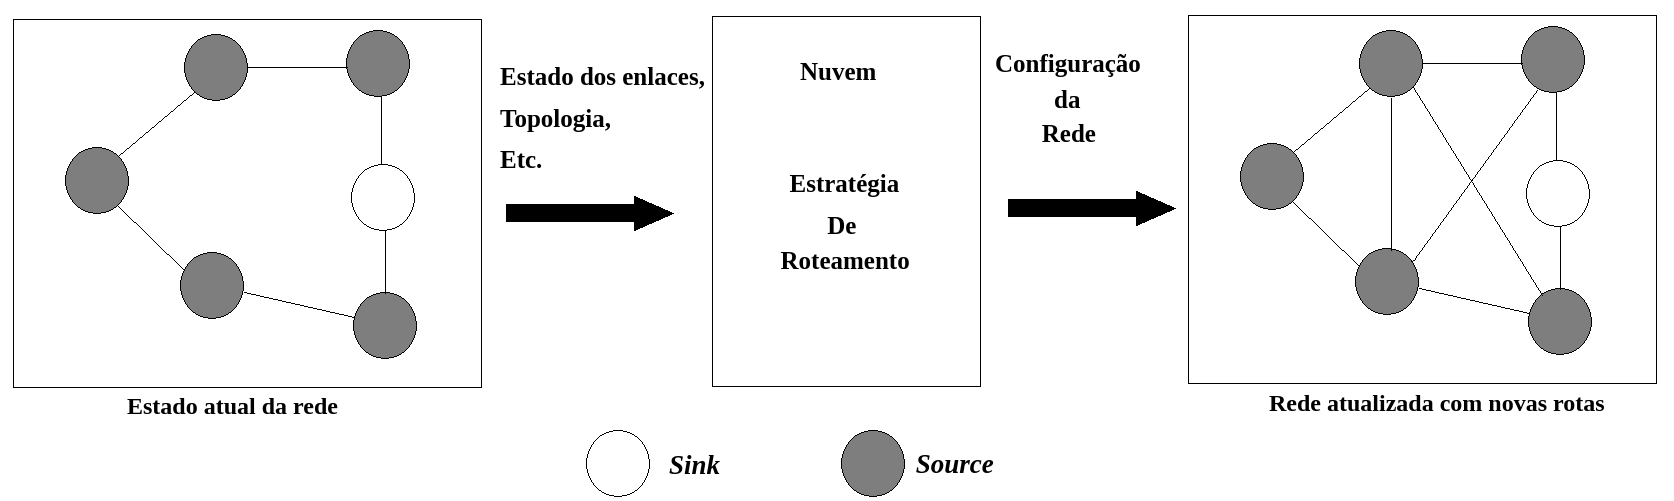
\includegraphics[width=15cm]{figs/overviewDoSistema.png}
    \caption{Modelo do sistema.}
    \label{modeloDoSistema}
\end{figure}

\section{Objetivos Gerais}
\label{s_introducao_OG}

O objetivo geral deste trabalho é implementar uma rede de sensores sem fio, baseada no conceito de Redes Definidas por Software (SDN) com fins de atender aos requisitos de \ac{QoS} das aplicações que se executam sobre a \ac{RSSF}.

\section{Objetivos específicos}
\label{s_introducao_OE}
\begin{itemize}
  \item Implantar e analisar o comportamento de uma aplicação sobre a plataforma \ac{SDN-WISE} no simulador Cooja e nos sensores Micaz;
  \item Conceber e implementar um controlador \ac{SDN} que possibilite construir regras de roteamento a partir de uma configuração estática dos módulos e, dos fluxos que possuem requisitos de \ac{QoS} associados à largura de banda e ao nível de bateria dos módulos;
  \item Implantar uma rede real com a aplicação definida anteriormente e avaliar o comportamento da mesma.
  \item Analisar algoritmos de roteamento para \ac{RSSF} e, adequá-los para o cumprimento de requisitos de \ac{QoS} referentes à vazão e consumo energético das aplicações que executam sobre o \ac{SDN-WISE};
  \item Implementar as regras de roteamento em uma aplicação piloto, utilizando o simulador Cooja.
\end{itemize}
